\documentclass[paper=screen,mathserif]{beamer}\usepackage[]{graphicx}\usepackage[]{color}
%% maxwidth is the original width if it is less than linewidth
%% otherwise use linewidth (to make sure the graphics do not exceed the margin)
\makeatletter
\def\maxwidth{ %
  \ifdim\Gin@nat@width>\linewidth
    \linewidth
  \else
    \Gin@nat@width
  \fi
}
\makeatother

\definecolor{fgcolor}{rgb}{0.345, 0.345, 0.345}
\newcommand{\hlnum}[1]{\textcolor[rgb]{0.686,0.059,0.569}{#1}}%
\newcommand{\hlstr}[1]{\textcolor[rgb]{0.192,0.494,0.8}{#1}}%
\newcommand{\hlcom}[1]{\textcolor[rgb]{0.678,0.584,0.686}{\textit{#1}}}%
\newcommand{\hlopt}[1]{\textcolor[rgb]{0,0,0}{#1}}%
\newcommand{\hlstd}[1]{\textcolor[rgb]{0.345,0.345,0.345}{#1}}%
\newcommand{\hlkwa}[1]{\textcolor[rgb]{0.161,0.373,0.58}{\textbf{#1}}}%
\newcommand{\hlkwb}[1]{\textcolor[rgb]{0.69,0.353,0.396}{#1}}%
\newcommand{\hlkwc}[1]{\textcolor[rgb]{0.333,0.667,0.333}{#1}}%
\newcommand{\hlkwd}[1]{\textcolor[rgb]{0.737,0.353,0.396}{\textbf{#1}}}%

\usepackage{framed}
\makeatletter
\newenvironment{kframe}{%
 \def\at@end@of@kframe{}%
 \ifinner\ifhmode%
  \def\at@end@of@kframe{\end{minipage}}%
  \begin{minipage}{\columnwidth}%
 \fi\fi%
 \def\FrameCommand##1{\hskip\@totalleftmargin \hskip-\fboxsep
 \colorbox{shadecolor}{##1}\hskip-\fboxsep
     % There is no \\@totalrightmargin, so:
     \hskip-\linewidth \hskip-\@totalleftmargin \hskip\columnwidth}%
 \MakeFramed {\advance\hsize-\width
   \@totalleftmargin\z@ \linewidth\hsize
   \@setminipage}}%
 {\par\unskip\endMakeFramed%
 \at@end@of@kframe}
\makeatother

\definecolor{shadecolor}{rgb}{.97, .97, .97}
\definecolor{messagecolor}{rgb}{0, 0, 0}
\definecolor{warningcolor}{rgb}{1, 0, 1}
\definecolor{errorcolor}{rgb}{1, 0, 0}
\newenvironment{knitrout}{}{} % an empty environment to be redefined in TeX

\usepackage{alltt}

\usetheme{CambridgeUS} 
\useinnertheme{circles}
\useoutertheme[footline=authortitle,subsection = false]{miniframes}
%\useoutertheme{infolines}
\setbeamercolor{palette tertiary}{fg=white, bg=white!42!black}
\setbeamercolor{alerted text}{fg=red!73!black}

%%%%%%
\usepackage{natbib}     % for references
\usepackage[osf]{sourcesanspro}
\usepackage{sourcecodepro}
\usepackage{booktabs}
\usepackage{eulervm}
\usepackage{import}
\usepackage{prodint}
\usepackage{bbm}
\usepackage{tabularx}
\usepackage{dcolumn}
\usepackage{color}
\usepackage{booktabs}
\usepackage{graphicx,rotating,epsfig,multirow,multicol,hhline}
\usepackage{amsmath,amsthm,amssymb,amsfonts}
\newcommand{\subfloat}[2][need a sub-caption]{\subcaptionbox{#1}{#2}}




%% \usepackage{listings}
%% \lstset{
%%   basicstyle=\tiny\ttfamily, % Standardschrift
%%   % numbers=left,               % Ort der Zeilennummern
%%   %numberstyle=\tiny,          % Stil der Zeilennummern
%%   % stepnumber=2,               % Abstand zwischen den Zeilennummern
%%   numbersep=5pt,              % Abstand der Nummern zum Text
%%   tabsize=2,                  % Groesse von Tabs
%%   extendedchars=true,         %
%%   breaklines=true,            % Zeilen werden Umgebrochen
%%   keywordstyle=\color{blue},
%%   frame=b,         
%%   stringstyle=\color{white}\ttfamily, % Farbe der String
%%   showspaces=false,           % Leerzeichen anzeigen ?
%%   showtabs=false,             % Tabs anzeigen ?
%% }

\usepackage{subcaption}

\newcommand{\ft}[1]{\frametitle{#1}}
\newcommand{\fst}[1]{\framesubtitle{#1}}


\title{Introduction to biostatistical computing}
\institute[]{\scriptsize{\url{arthur.allignol@uni-ulm.de}}}

\date{}
%%%%%%

\makeatletter
\setbeamertemplate{footline}
{
  \leavevmode%
  \hbox{%
  \begin{beamercolorbox}[wd=.333333\paperwidth,ht=2.25ex,dp=1ex,center]{author in head/foot}%
    \usebeamerfont{author in head/foot}\insertshortauthor%~~\beamer@ifempty{\insertshortinstitute}{}{(\insertshortinstitute)}
  \end{beamercolorbox}%
  \begin{beamercolorbox}[wd=.333333\paperwidth,ht=2.25ex,dp=1ex,center]{title in head/foot}%
    \usebeamerfont{title in head/foot}\insertshorttitle
  \end{beamercolorbox}%
  \begin{beamercolorbox}[wd=.333333\paperwidth,ht=2.25ex,dp=1ex,right]{date in head/foot}%
    \usebeamerfont{date in head/foot}\insertshortdate{}\hspace*{2em}
    \insertframenumber\hspace*{2ex} 
  \end{beamercolorbox}}%
  \vskip0pt%
}
\makeatother

\AtBeginSection[]
{
  \begin{frame}
    \frametitle{Table of Contents}
    \tableofcontents[currentsection]
  \end{frame}
}
\IfFileExists{upquote.sty}{\usepackage{upquote}}{}
\begin{document}

% \newcommand{\onlyframenumber}{yes}

%%%%%% title page
\newcommand{\titlep}{yes}  % for titlepagelayout

{
\renewcommand{\insertframenumber}{}   % no page number on titlepage
\begin{frame}
\addtocounter{framenumber}{-1}
\titlepage
\end{frame}
}
%%%%%%


\frame{\tableofcontents[currentsection]}

\section{Reproducible Research}

\subsection{What is Reproducibility}

\begin{frame}
  \frametitle{Reproducible Research: A General Definition}
  Research results are {\em replicable} if there is enough information
  to enable an independent researcher to make the same findings using
  the same procedures.
  \begin{itemize}
  \item This is the aim of science
  \item Concept closely related to the concepts of replicability and
    generalisation
  \end{itemize}
  This definition is too general for us. We will aim for {\em
    reproducible analysis}, i.e., 
  
  \begin{center}
    ``the data and code used to make a
    finding are available and are sufficient for an independent
    researcher to recreate the findings''
  \end{center}
\end{frame}

\subsection{Reproducible Analysis}

\begin{frame}
  \frametitle{Reproducible Analysis} 

  What role can we play as (bio)statistician in reproducible
  research?\pause
  
  \vspace{1cm}
  We can at least aim for {\em reproducible analysis}
  \begin{itemize}
  \item The data and code used to make the findings are available and
    are sufficient for an independent researcher to recreate the
    findings
  \item I.e., from the raw data to the publications in well documented
    steps
  \end{itemize}\vspace{0.5cm}
  That ain't full reproducibility, but it's already something
\end{frame}

\begin{frame}
  \frametitle{Reproducible Analysis}
  {\em An article about computational science in a scientific
    publication is not the scholarship itself, it is merely advertising
    of the scholarship. The actual scholarship is the complete software
    development environment and the complete set of instructions which
    generated the figures.}\\
  --- D. Donoho
  
  \begin{itemize}
  \item The concept of reproducible research is based on the idea of
    {\em literate programming} such that the logic of the analysis is
    clearly represented in the final product by combining computer
    code/programs with ordinary human language
    
    $\Rightarrow$ Combine analysis code and report
  \end{itemize}
\end{frame}


\begin{frame}
  \frametitle{Data analysis work}
  \begin{enumerate}
  \item Data cleaning
    \begin{itemize}
    \item Data entry errors
    \item Missing data
    \item Recoding
    \end{itemize}
  \item Data transformation
    \begin{itemize}
    \item Transform variables
    \item Create new variables
    \item Reshape the data entirely to fit some models
    \end{itemize}
  \item Statistical analysis (incl. tables, graphs)
  \item Statistical report; publication
  \end{enumerate}
\end{frame}

\begin{frame}
  \frametitle{Research Work, e.g., Master thesis}
  \begin{enumerate}
  \item A new model (some maths)
  \item Program new model (in R)
  \item Simulation study to see whether asymptotic results translate
    in the real world (small sample properties)
  \item Illustrate the usefulness of the new approach with some data
  \item Publication; talks
  \end{enumerate}
\end{frame}

\begin{frame}
  \frametitle{Reproducible Analysis: Barriers/Disadvantages}
  \begin{itemize}
  \item Awareness
  \item Find the right tools
  \item Learn new tools
  \item More work from the start
  \end{itemize}
  \pause\vspace{0.6cm}
  Benefits outweigh the disadvantages  
\end{frame}

\begin{frame}
  \frametitle{Reproducible Analysis: Benefits}
  \framesubtitle{For science:}
\begin{itemize}
\item Reproducibility is a key part of scientific inquiry
\item Reproducibility permits to evaluate scientific claims
\item Avoids effort duplication and encourage cumulative knowledge
  development
\end{itemize}
Examples:
\begin{itemize}
\item A colleague wants to try out your new model
\item Somebody wants to compare your approach to hers in your
  simulation setting 
\end{itemize}
\end{frame}

\begin{frame}
  \frametitle{Reproducible Analysis: Benefits}
  \framesubtitle{For you:}
  Better work habits
  \begin{itemize}
  \item Making a project reproducible from the start encourages you to
    use better work habits
    \begin{itemize}
    \item better organisation
    \item better code quality if you think that somebody might
      actually have a look at it 
    \end{itemize}
  \end{itemize}
  Examples:
  \begin{itemize}
  \item Perform some supplementary analyses within the review process
    of a paper
  \end{itemize}
\end{frame}

\begin{frame}
  \frametitle{Reproducible Analysis: Benefits}
  \framesubtitle{For you:}
  \begin{center}
    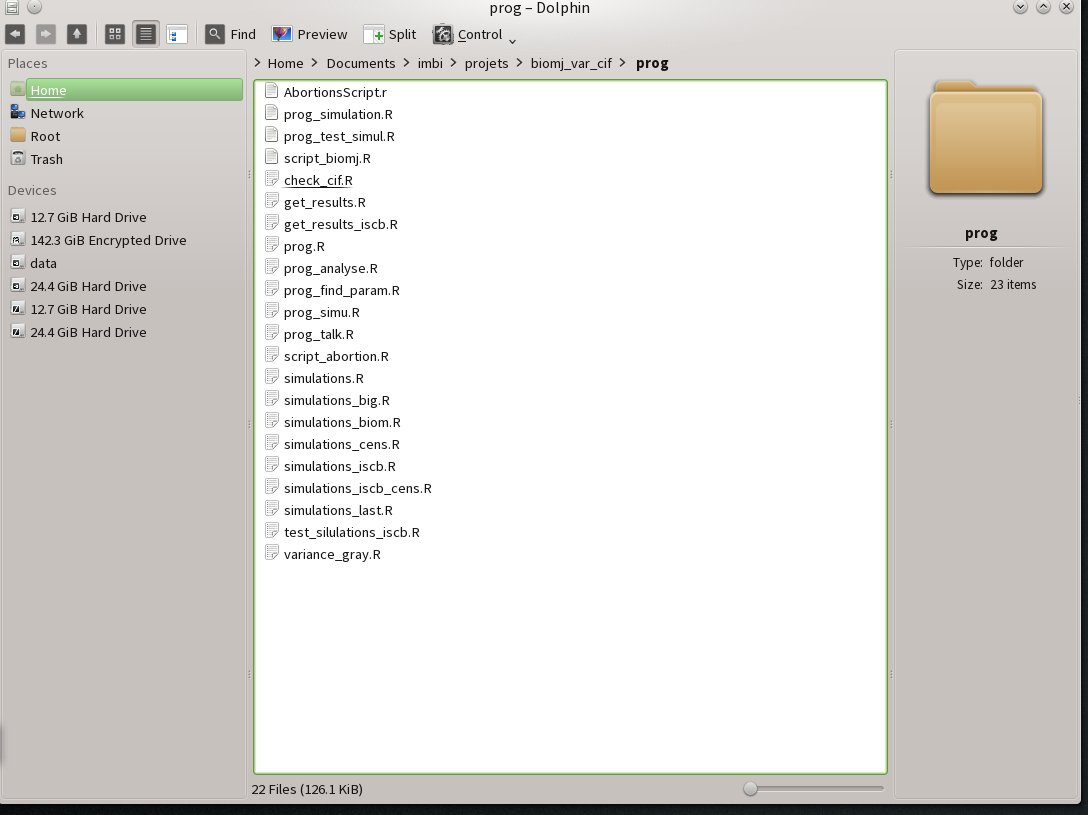
\includegraphics[width = \linewidth]{graphics/folders.jpeg}
  \end{center}
\end{frame}

\begin{frame}
  \frametitle{Reproducible Analysis: Benefits}
  \framesubtitle{For you:}
  Changes are {\bf a lot} easier
  \begin{itemize}
  \item Data analysis is done but the doctors messed up with $Z$.\\
    They are sending you a new data set
  \item $Z$ is included in a lot of regression models
  \item You did the data transformation in excel $\rightarrow$ no
    trace of it
  \item You copy/pasted the results of the regression models from the
    R/SAS console in a Word document
  \item Worst-case scenario: you used point and click software (e.g., SPSS)
  \item It's Friday 5pm, the results {\bf have} to be available on Monday 8am
  \end{itemize}
  $\Rightarrow$ Have a nice weekend!
\end{frame}

\begin{frame}
  \frametitle{Reproducible Analysis: Benefits}
  Better teamwork
  \begin{itemize}
  \item If an independent researcher can reproduce your analysis, so
    can a collaborator
  \item That applies to both current and future collaborators
  \end{itemize}
  Higher research impact
  \begin{itemize}
  \item Reproducible research more useful for other researchers
  \end{itemize}\pause
  Some more pragmatic reasons
  \begin{itemize}
  \item We use computers more and more; Quality Assurance processes
    from the software engineering will come to us
  \item {\bf My} prediction is that reproducible analysis will become
    mandatory in the close future
  \end{itemize}
\end{frame}

\subsection{The tools of reproducible research}

\begin{frame}
  \frametitle{The Tools of Reproducible Research}
  \begin{itemize}
  \item A good statistical software that actually permits to write
    code: {\bf R}, {\bf SAS}, Stata
  \item {\em Literate programming}: Combine code with text in a single
    file
    \begin{itemize}
    \item ODS (Output Delivery System) in SAS
    \item {\bf Sweave} and {\bf knitr} packages in R
    \end{itemize}
  \item Markup languages, e.g., \LaTeX, HTML, Markdown
  \item A good editor (e.g., Rstudio)
  \item Some good programming practice, i.e., comments, meaningful
    variable names
  \end{itemize}\pause
  Optional but very useful
  \begin{itemize}
  \item Version control software
  \item Shell scripting abilities (for bigger projects)
  \end{itemize}
\end{frame}

\begin{frame}
  \frametitle{Statistical Software}
  The way you interact with R, SAS, Stata or other programming
  languages has benefits for reproducible research
  \begin{itemize}
  \item Interaction with the language by explicitely writing down your
    steps as source code
  \item A lot better than point and click programs for reproducible
    research
    \begin{itemize}
    \item Your steps are usually lost when you click around to fit
      models 
    \end{itemize}
  \item {\em Literate programming} only possible with source code
  \end{itemize}
\end{frame}

\begin{frame}
  \frametitle{Literate Programming} ``Literate programming is an
  approach to programming introduced by Donald Knuth (1970s) in which
  a program is given as an explanation of the program logic in a
  natural language, such as English, interspersed with snippets of
  macros and traditional source code, from which a compilable source
  code can be generated'', i.e., {\em writing documentation containing
    computer code}
  \vspace{0.3cm}\pause
  \begin{itemize}
  \item For statistician it means being able to
    \begin{itemize}
    \item combine programming code with report text (article,
      presentation) in a single self-documenting file
    \item document the code and its results, including interpretation
      of the results
    \item allow an analysis to be rerun and the report (article,
      presentation) to be re-typeset by running a single command
    \end{itemize}
   \end{itemize}
\end{frame}

\begin{frame}
  \frametitle{Literate Programming}
  In R
  \begin{itemize}
  \item The {\bf Sweave} package: Embed R code in \LaTeX{} files. A
    pass through Sweave converts the file to a {\tt .tex} file, in which
    code, tables, graphics are included 
  \item The {\bf knitr} package: An evolution of {\bf Sweave}. {\bf
      knitr} adds some useful features and permits additionally to
    embed R code in html and markdown documents
  \item Plenty of useful packages that creates markup tables from,
    e.g., model fit
  \end{itemize}
  In SAS
  \begin{itemize}
  \item SASweave: SAS code in \LaTeX
  \item ODS: Output SAS ``stuffs'' in various file format (pdf, rtf,
    html, ...)
  \end{itemize}
\end{frame}

\begin{frame}[fragile]
  \frametitle{Good coding practice}
  {\em Comments}
  \begin{itemize}
  \item Text in the code that are not compiled/executed by the program
  \item Explain what difficult pieces of code do, e.g.,
\begin{knitrout}\scriptsize
\definecolor{shadecolor}{rgb}{0.969, 0.969, 0.969}\color{fgcolor}\begin{kframe}
\begin{alltt}
\hlkwa{for} \hlstd{(i} \hlkwa{in} \hlkwd{seq_along}\hlstd{(times)) \{}
    \hlstd{dna[}\hlkwd{cbind}\hlstd{(ii, ii, i)]} \hlkwb{<-} \hlopt{-}\hlstd{(}\hlkwd{.rowSums}\hlstd{(nev[, , i],} \hlkwd{dim}\hlstd{(nev)[}\hlnum{1}\hlstd{],}
                                        \hlkwd{dim}\hlstd{(nev)[}\hlnum{1}\hlstd{],} \hlnum{FALSE}\hlstd{))} \hlopt{/}
        \hlstd{nrisk[i, ]}
\hlstd{\}}
\end{alltt}
\end{kframe}
\end{knitrout}

{\scriptsize
\begin{verbatim}
\end{verbatim}}
  \end{itemize}
  {\em Meaningful variable names}
  \begin{itemize}
  \item {\tt temp1}, {\tt temp2}, etc. are not good
  \item {\tt Horrible\_Disease} with value {\tt Yes} and {\tt No} is
    better
  \end{itemize}
{\em Header}
\begin{itemize}
\item Write as a comment the aim of the program, your name and email
  at the beginning of the file 
\end{itemize}
{\em Good file organisation} 
\end{frame}

\begin{frame}
  \frametitle{A good Editor}
  \begin{itemize}
  \item Auto-completion is an extremely useful feature, especially
    when using meaningful (long) variable names.
  \item Rstudio is a good R editor
    \begin{itemize}
    \item Good interaction with markup languages
    \item Interaction with version control systems
    \item Using {\bf Sweave} or {\bf knitr} is made easy
    \end{itemize}
  \end{itemize}
\end{frame}

\begin{frame}
  \frametitle{Advanced Tools: Version Control and Shell}
  Version Control
  \begin{itemize}
  \item Practice that tracks and provides control over changes to
    files (e.g., source code)
  \item Example: Git
  \end{itemize}
  Shell scripts
  \begin{itemize}
  \item When projects get big, having everything in one file is
    actually a problem
  \item Shell scripts permit to ``glue'' several analyses together
  \item Example: A single shell script executes separated R programs
  \end{itemize}
\end{frame}

\begin{frame}
  \frametitle{But...}
  Perfect reproducibility is not achievable
  \begin{itemize}
  \item Differences in
    \begin{itemize}
    \item Operating systems
    \item Processors
    \item Software and package versions
    \item \dots
    \end{itemize}
  \end{itemize}
\end{frame}

\section{Real Life Data}

\begin{frame}[fragile]
  \ft{Real Life Data}
\begin{knitrout}\scriptsize
\definecolor{shadecolor}{rgb}{0.969, 0.969, 0.969}\color{fgcolor}\begin{kframe}
\begin{alltt}
\hlkwd{library}\hlstd{(fortunes)}
\hlkwd{fortune}\hlstd{(}\hlstr{"Tolstoy"}\hlstd{)}
\end{alltt}
\begin{verbatim}
## 
## Happy families are all alike; every unhappy family is
## unhappy in its own way.
## Leo Tolstoy
## 
## and every messy data is messy in its own way - it's easy to
## define the characteristics of a clean dataset (rows are
## observations, columns are variables, columns contain values
## of consistent types). If you start to look at real life
## data you'll see every way you can imagine data being messy
## (and many that you can't)!
##    -- Hadley Wickham (answering 'in what way messy data
##       sets are messy')
##       R-help (January 2008)
\end{verbatim}
\end{kframe}
\end{knitrout}
\end{frame}

\begin{frame}
  \begin{center}
    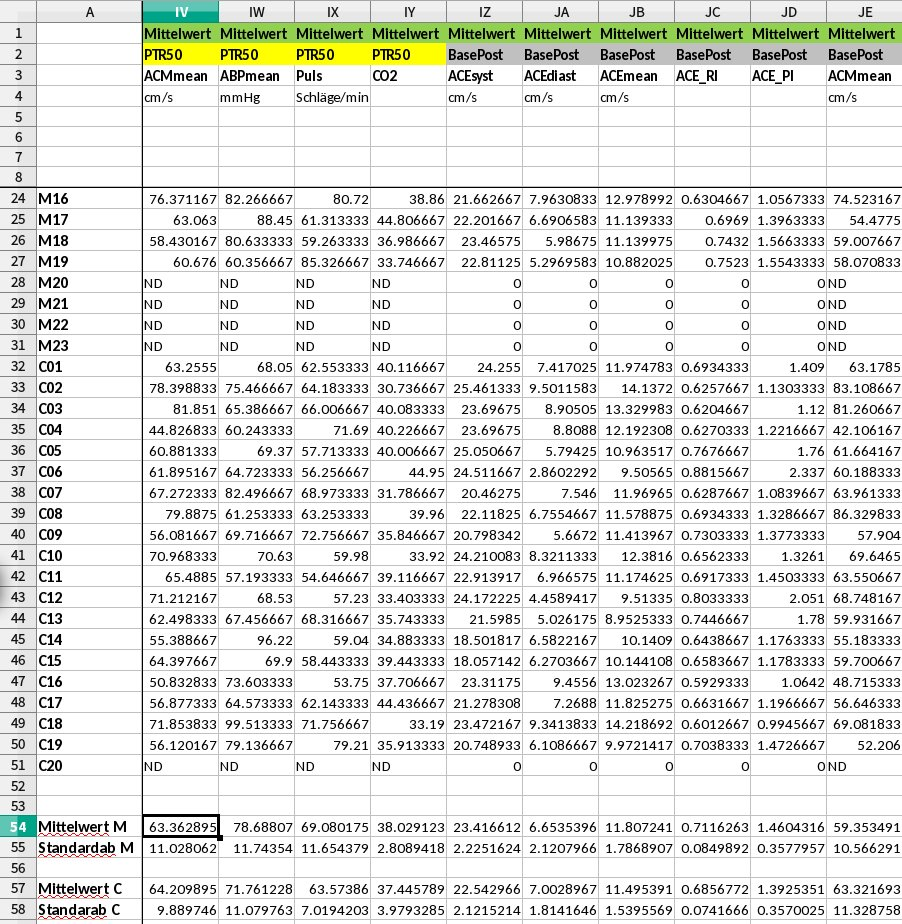
\includegraphics[width=8cm]{graphics/real_life_data2.jpeg}
  \end{center}
\end{frame}

\begin{frame}
  \ft{Real Life Data}
  {\em The problems}
  \begin{itemize}
  \item Bad structure
  \item Non ascii characters (e.g., Umlaut)
  \item Variable names with spaces; on several lines, \dots
  \item Colour coding
  \item No consistent definition of missing values
  \item Free text
  \item (Wrong input, e.g., person who die twice)
  \item \dots
  \end{itemize}\pause
  Often data need to be transformed/reshaped for fitting a particular model
\end{frame}

\begin{frame}
  \ft{Real Life Data}
  
  {\em The tools needed}
  \begin{itemize}
  \item Read data
  \item Work with strings/characters variables
  \item Factors and dates
  \item Data manipulation, reshaping, merging
  \end{itemize}

\end{frame}

\section{Simulation Studies}

\begin{frame}
  \frametitle{Simulation Studies}
  What is a simulation study?
  \begin{description}
  \item[Simulation] A numerical technique for conducting experiments
    on the computer
  \item[Monte Carlo simulation] Computer experiment that involves
    random sampling from probability distributions
    \begin{itemize}
    \item {\bf Extremely} useful in statistics
    \item When a statistician talks about simulation, it usually means
      Monte Carlo simulation
    \end{itemize}
  \end{description}
\end{frame}


\begin{frame}
  \frametitle{Simulation Studies}
  Why do we do simulation studies?
  \begin{itemize}
  \item Properties of statistical methods should be established,
  \item but analytical derivations rarely possible
  \item Large sample approximations of these properties are possible
  \item but at the end of the day, we need to evaluate the methods in
    (finite) sample sizes that are likely to be seen in practice
  \item Analytical results usually require assumptions
  \item We also need to know what happens when these assumptions are
    violated
    \begin{itemize}
    \item Extremely difficult to do analytically
    \end{itemize}
  \end{itemize}
\end{frame}

\begin{frame}
  \frametitle{Simulation Studies} Simulation studies permit, under
  various conditions, to answer questions like
  \begin{itemize}
  \item What is the bias of an estimator in finite samples
  \item Is this estimator still consistent under departures from the
    assumptions
  \item How does a new statistic compare to competing ones in terms of
    bias, precision
  \item Does the procedure for constructing a confidence interval for
    a parameter achieve the nominal level of coverage
  \end{itemize}
This questions cannot usually be answered analytically
\end{frame}

\begin{frame}
  \frametitle{Simulation Studies}
How does that work?
\begin{enumerate}
\item Generate $S$ independent data sets under the condition of interest
\item Compute the numerical value of the statistic of interest $T$ for
  each data set. We obtain $T_1, T_2, \dots, T_S$
\item If $S$ large enough (say, 1000), summary statistics across $T_1,
  T_2, \dots, T_S$ is a good approximation to the true sampling
  properties of the statistic under the conditions of interest
\end{enumerate}
\end{frame}

\begin{frame}
  \frametitle{Simulation Studies}
  What we will learn?
  \begin{itemize}
  \item Generate realistic data sets
  \item Summarise simulation results in some intelligible way
  \item If time permits: Parallelisation
  \end{itemize}
\end{frame}

\section{Further Topics}

\begin{frame}
  \ft{Further Topics}
  \fst{Graphics}
  
  {\bf Why do we need graphics?}
  \begin{itemize}
  \item Data exploration
    \begin{itemize}
    \item Look for trends and/or associations between variable
    \item The first step before modelling
    \item $\rightarrow$ quick and dirty graphs
    \end{itemize}
  \item Check assumptions of statistical models
  \item These graphics are usually for you
  \end{itemize}
\end{frame}

\begin{frame}
  \ft{Further Topics}
  \fst{Graphics}
  
  {\bf Why do we need graphics?}
  \begin{itemize}
  \item Information visualisation/Communication
    \begin{itemize}
    \item Need a lot of polishing
    \item Iteration is crucial
    \item Think about where you present the graphics, e.g, colour,
      line thickness for a beamer presentation
    \end{itemize}
  \end{itemize}
\end{frame}

\begin{frame}
  \ft{Minard's Flow Map}
  \centering
  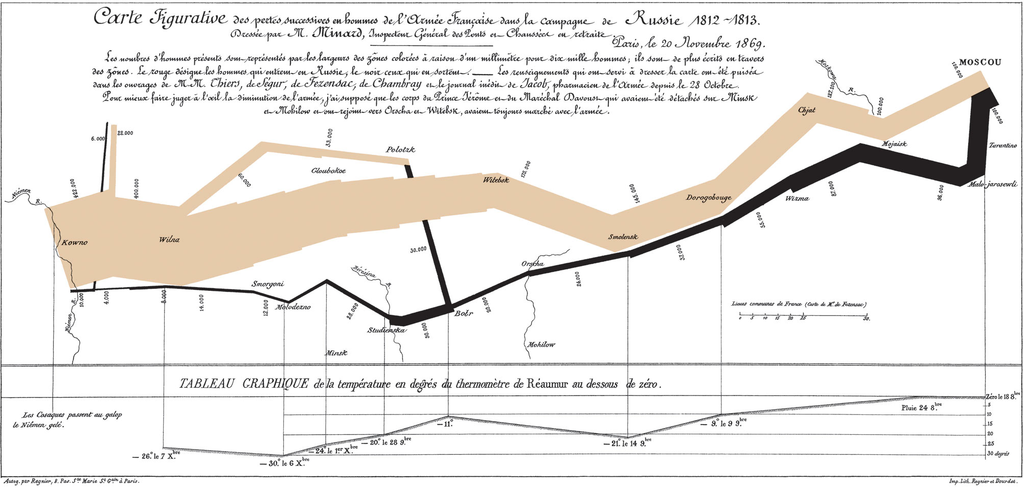
\includegraphics[width=\linewidth]{graphics/1024px-Minard.png}
\end{frame}

\begin{frame}
  \ft{Further Topics}
  \begin{itemize}
  \item Debugging
  \item Something you might want to hear about?
  \end{itemize}
\end{frame}

\end{document}
